%\documentclass{article}
%
\newcommand{\Linh}{9}
\newcommand{\Colun}{3}
%\title{Manual de instalação do quadro terminal}
%\author{Mundo LED}
%
%\begin{document}

%\maketitle
%%\chapter{Manual de instalação do quadro terminal}

\chapter{Manual de instalação do quadro terminal \Linh X\Colun}
%\section{introducao.tex}
Visão geral do manual e do quadro de comando. 
Lista de verificação dos materiais necessários.
Manual para instalação do Quadro Terminal para Painel Led Full Color 9 x 3 m.
\begin{figure}
\centering
\begin{subfigure}{0.4\textwidth}
	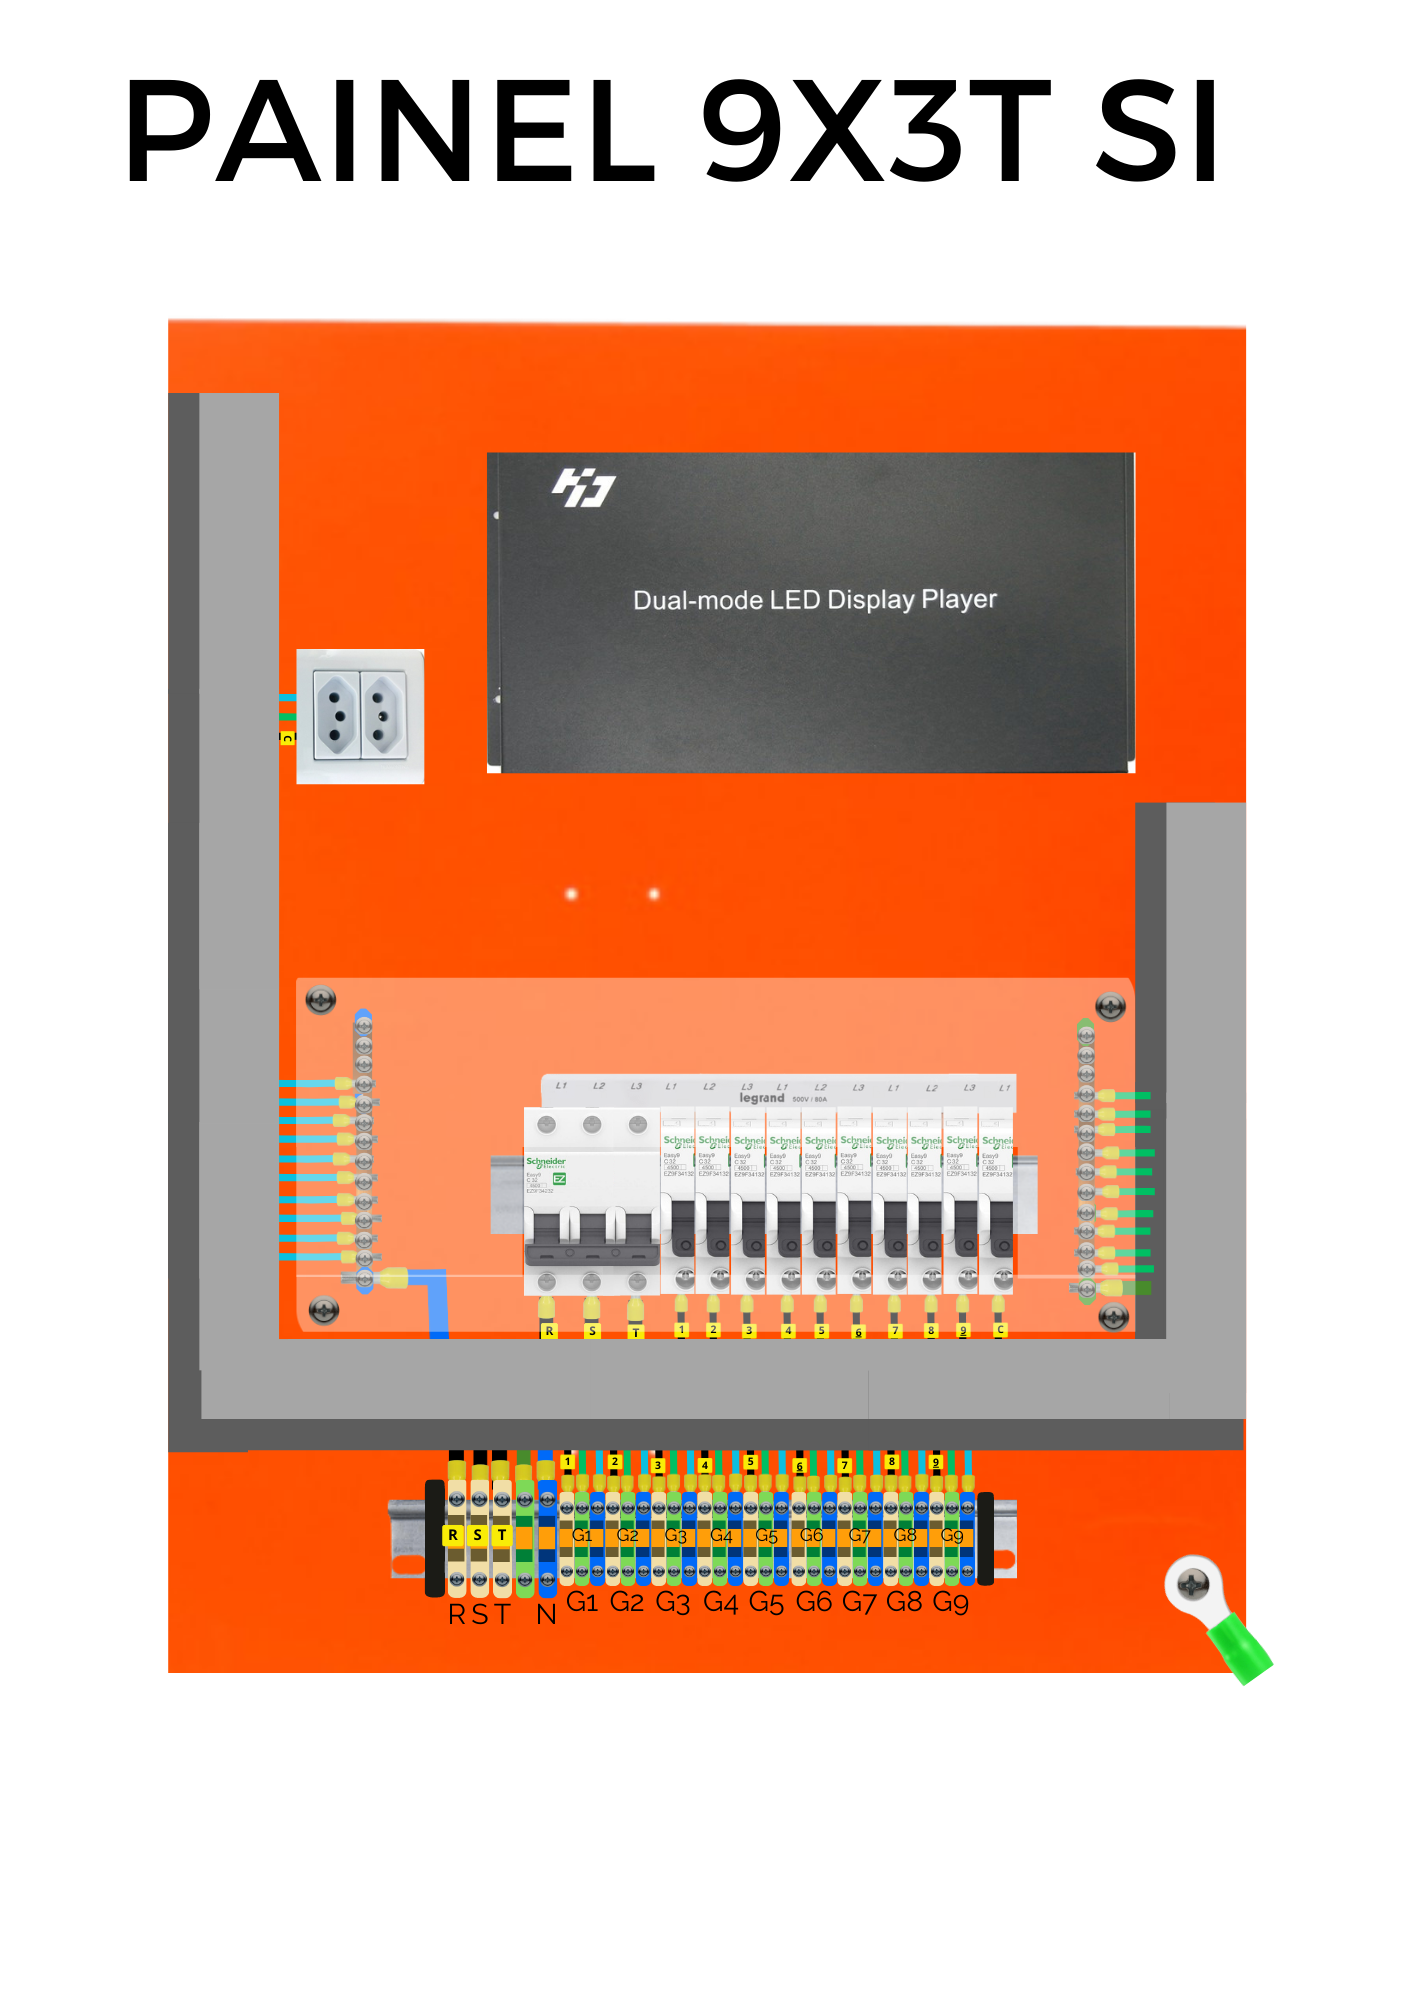
\includegraphics[width=\textwidth]{image/9.png}
	\caption{Quadro terminal para painel simples interno 9x3.}
	\label{fig:advQD_1}
\end{subfigure}
\hfill
\begin{subfigure}{0.4\textwidth}
    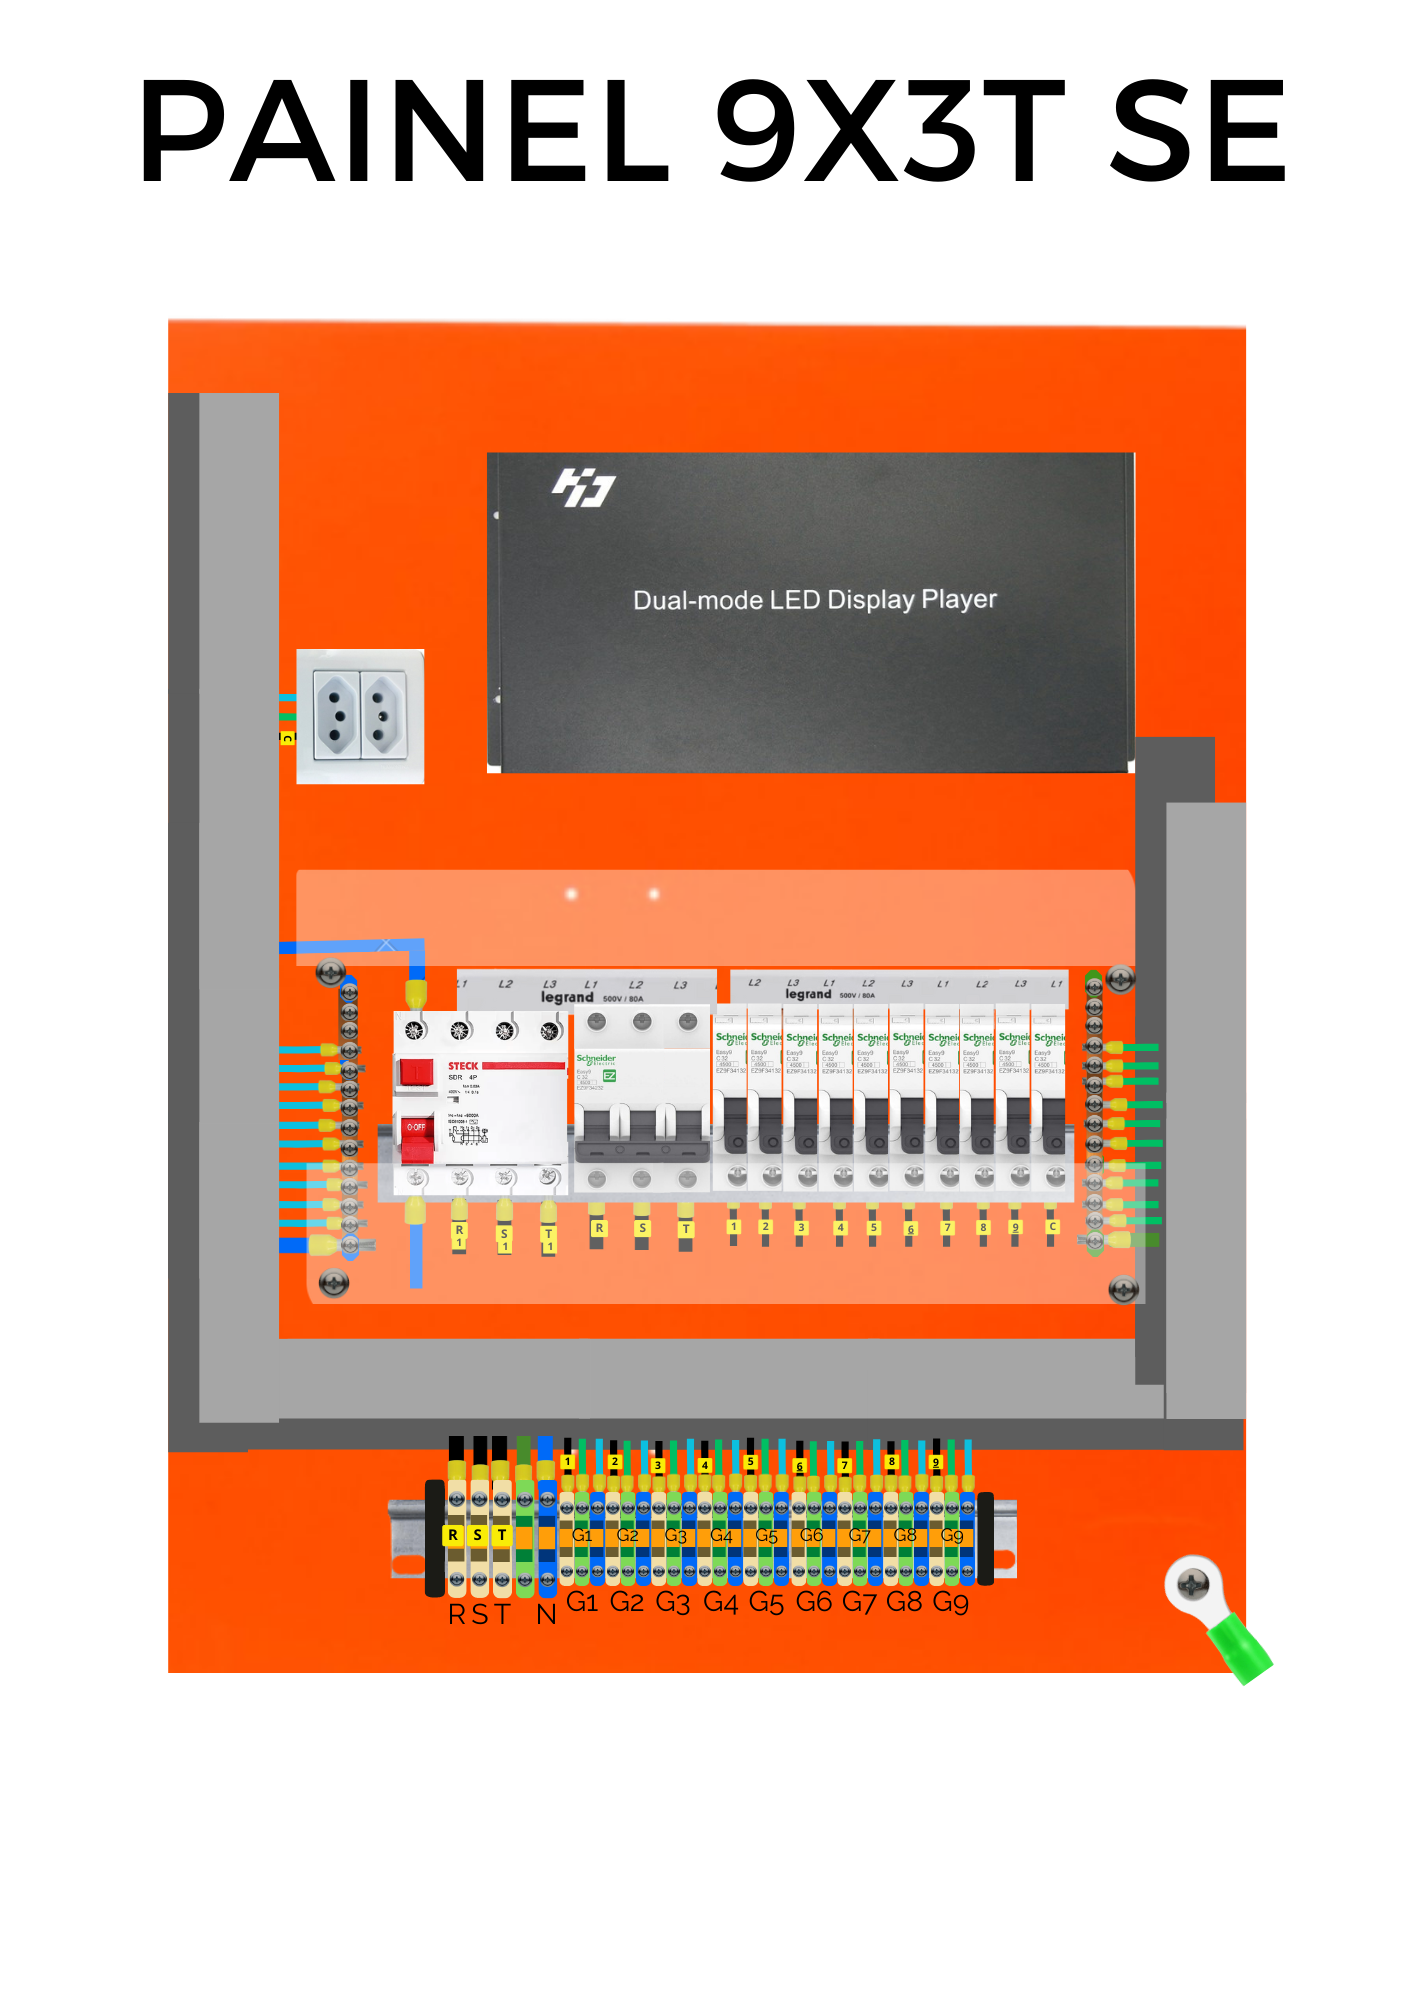
\includegraphics[width=\textwidth]{image/10.png}
    \caption{Quadro terminal para painel simples externo 9x3.}
    \label{fig:advQD_2}
\end{subfigure}
\begin{subfigure}{0.4\textwidth}
    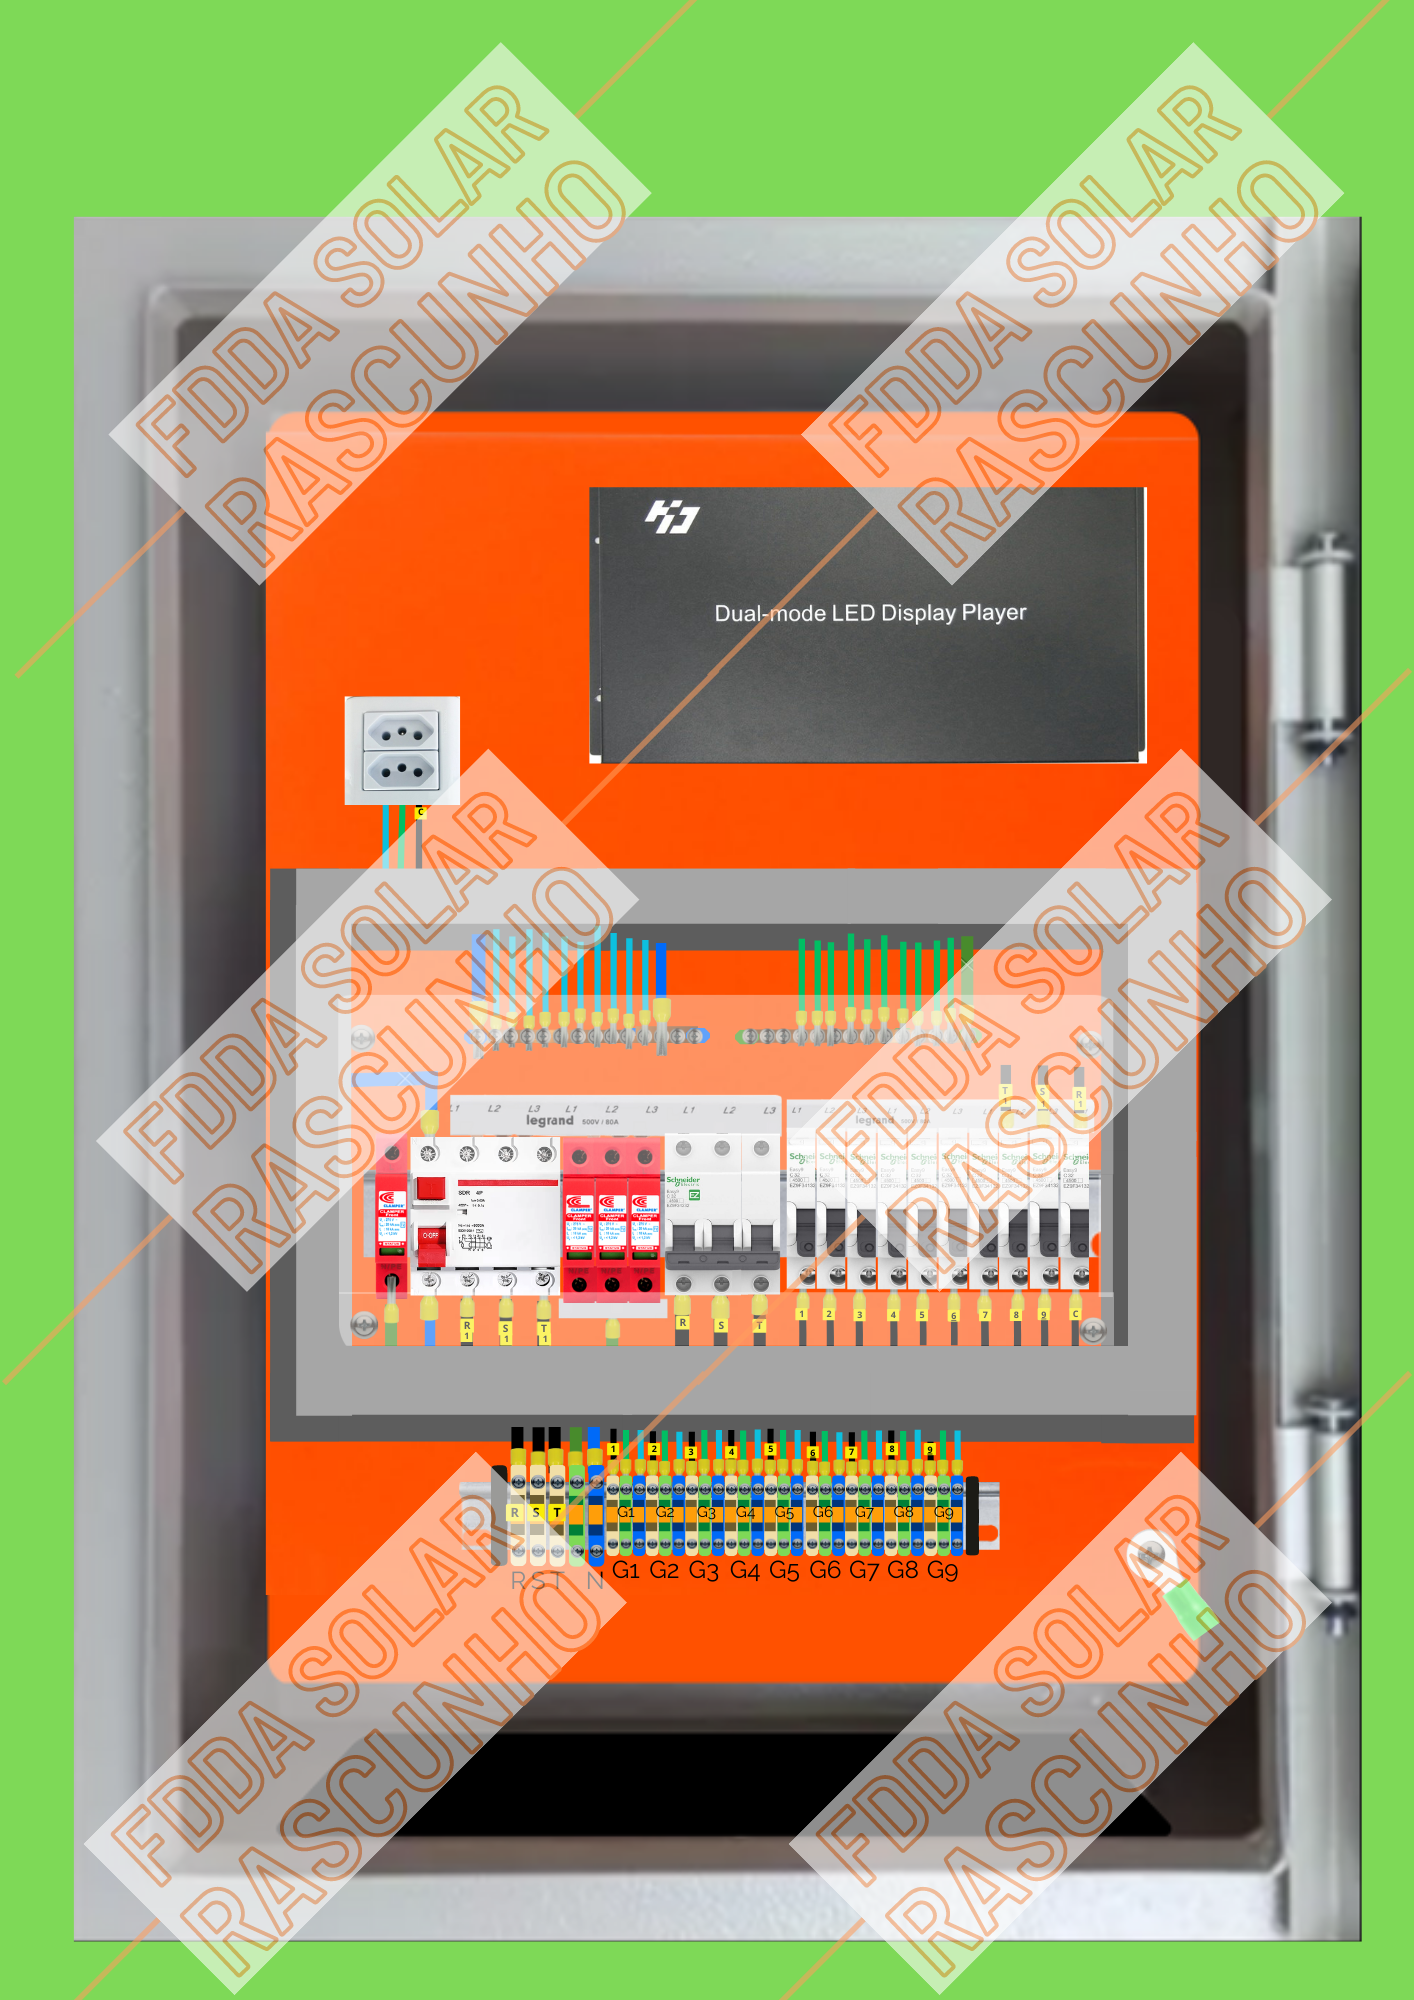
\includegraphics[width=\textwidth]{image/3.png}
    \caption{Quadro terminal para painel completo externo 9x3.}
    \label{fig:advQD_2}
\end{subfigure}
\caption{Quadro terminal para painel 9x3.}
\label{fig:advQD}
\end{figure}

queda de tensão $<0,5%$


\section{Preparação do local}
O local onde ficará o quadro deve ser escolhido visando garantir a segurança e eficiência em seu funcionamento. 
O quadro terminal deverá ficará próximo ao painel em distância menor que 5 m, caso não seja possível, ajustar a distância máxima entre o quadro terminal e o quadro de distribuição geral.
A fonte de alimentação elétrica deve ser de preferencia a partir do quadro de distribuiçao geral, em circuito único e dedicado. Ou que os cabos de alimentação, as proteções esteja dimensionados obedecando as normas de segurança.
Prepare infra estrutura elétrica entre a fonte e o local onde será instalado o quadro, observando as normas de segurança.
O espaço deve ser ventilado, evitar poeira e umidade conforme o grau de proteção IPXX do quadro.
O local deve ser de fácil acesso para os eletricistas, sem obstáculos ou objetos que possam interferir na manutenção do sistema.
O quadro deve ser instalado na posição vertical, em parede resistente e ou suporte adequado para garantir sua estabilidade e segurança.
 
 \begin{quote}
 Colocar as tabelas de carga dos conjuntos de gabinete, 1, 2, 3 e comunicação
 colocar informação da divisão de carga (melhor) com quanto carga será acrescentado em cada  fase. Informação para o cliente adequar o sistema se for necessário.
 \end{quote}

%\section{Montagem do quadro de comando}
Notas sobre cabos flexiveis (fios)
Seção mínima dos cabos determinada pela norma ABNT NBR 5410. As informações aqui são orientativas, baseadas nas condições mais usuais de instalação (B1) encontradas no país.

Dimensionamento de cabos deve ser realizado conforme norma ANBT NBR 5410. Como a corrente para alimentação do painel é superior a 10 A, o quadro deve ser atendido por um circuito exclusivo.
\begin{table}[htbp]
\caption{Proteção do condutor - capacidade de condução dos condutores conforme norma ABNT NM 247-3}
\begin{tabular}{|l|l|l|}
\hline
Seção nominal &  Capacidade de condução  & Disjuntor máximo \\ \hline
1,5 mm 2  & 15,5 A  & 10 A \\ \hline
2,5 mm 2  & 21 A  & 20 A \\ \hline
4 mm 2  & 28 A  & 25 A \\ \hline
6 mm 2  & 36 A  & 32 A \\ \hline
10 mm 2  & 50 A  & 50 A \\ \hline
16 mm 2  & 68 A  & 63 A \\ \hline
25 mm 2  & 89 A  & 80 A \\ \hline
\end{tabular}
\label{tab:disjuntorcabo}
\end{table}
 


\section{Instalação do quadro de comando}
\begin{description}
\item[ATENÇÃO] Somente conectar os cabos depois do quadro devidamente fixado no local. 
\end{description}

Fixação do quadro de comando no local escolhido. 

Conexão dos cabos de entrada e saída ao quadro de comando.
\begin{description}
\item[ATENÇÃO] Primeiro conectar as saídas para o painel e depois a entrada. Trabalhar com os cabos desenergizados. 
\end{description}
 
Instalação dos dispositivos de proteção (disjuntores, fusíveis, etc.).

\section{Teste e verificação}
Verificação da conexão elétrica e aterramento.
Verificação da operação dos componentes do quadro de comando (disjuntores, contatores, etc.). 
Verificação da configuração dos ajustes de proteção e controle. Verificação da tensão e corrente elétrica.

\section{Instruções de operação e manutenção}
Instruções para a operação do quadro de comando. Instruções para a manutenção e reparação do quadro de comando. Lista de verificação de manutenção preventiva.
\begin{description}
\item[ATENÇÃO] Os dispositivos de proteção existentes no quadro não devem ser substituido por outro tipo com caracteristica diferentes.Trocar por outro dispositivo pode gerar prejuízo a vida e ao patrimônio.  Em caso de necessidade de substituição chame um profissional eletricista habilitado. 
\end{description}

\section{Conclusão}
Resumo das etapas de instalação. Informações de suporte e contato. Agradecimentos e observações finais.
\section{Definições}
Definiçoes retiradas da NBR 5410
\begin{description}
\item[Quadro de distribuição principal] Primeiro quadro de distribuição após a entrada da linha elétrica na edificação.
\end{description}






%\end{document}
